% Title: gl2ps_renderer figure
% Creator: GL2PS 1.4.0, (C) 1999-2017 C. Geuzaine
% For: Octave
% CreationDate: Fri Jul 19 10:55:20 2024
\setlength{\unitlength}{1pt}
\begin{picture}(0,0)
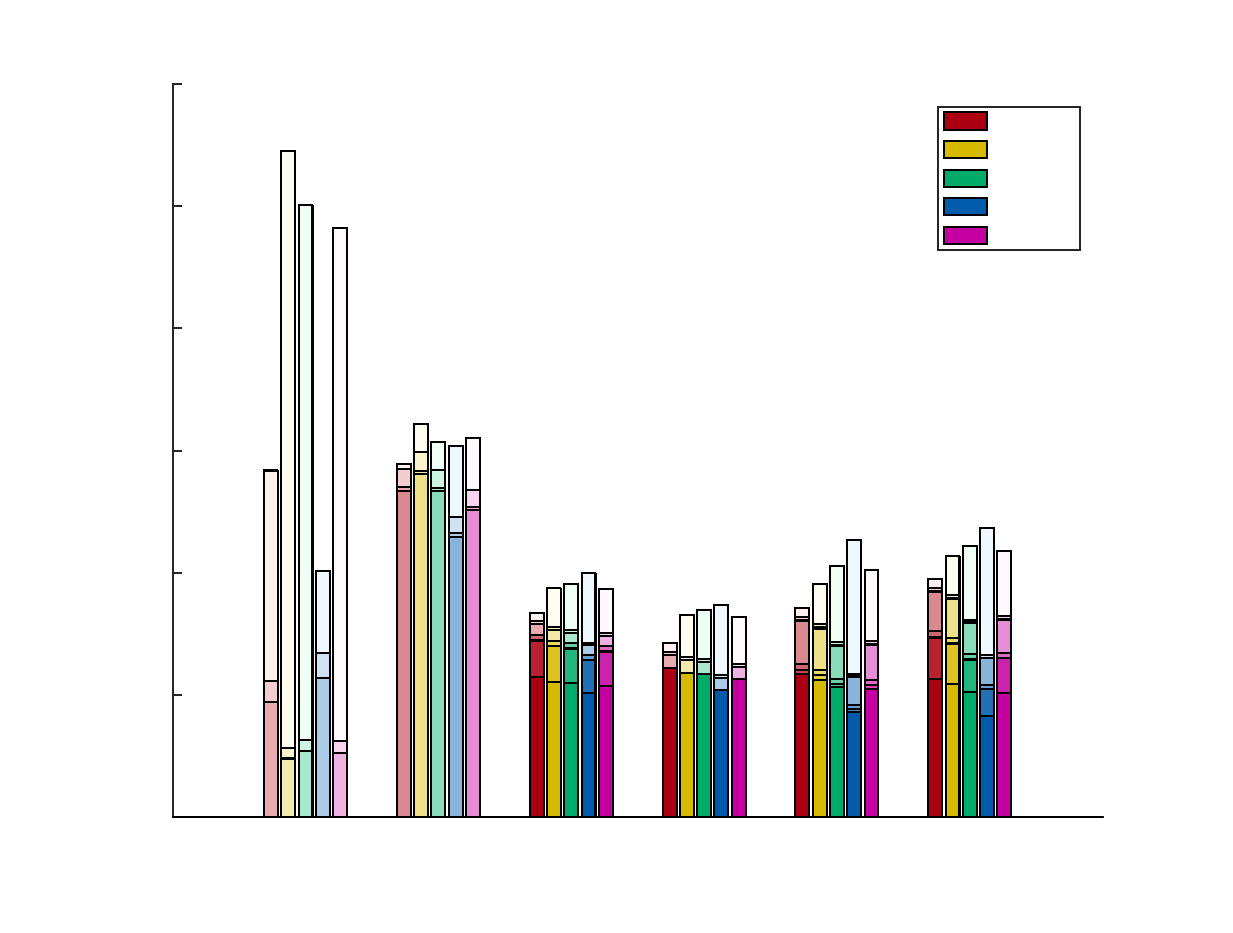
\includegraphics{results_plots/flur_times_full-inc}
\end{picture}%
\begin{picture}(576,432)(0,0)
\fontsize{10}{0}
\selectfont\put(138.651,40.0183){\makebox(0,0)[t]{\textcolor[rgb]{0.15,0.15,0.15}{{none-geo}}}}
\fontsize{10}{0}
\selectfont\put(202.423,40.0183){\makebox(0,0)[t]{\textcolor[rgb]{0.15,0.15,0.15}{{none-kdt}}}}
\fontsize{10}{0}
\selectfont\put(266.194,40.0183){\makebox(0,0)[t]{\textcolor[rgb]{0.15,0.15,0.15}{{kdt-geo}}}}
\fontsize{10}{0}
\selectfont\put(329.966,40.0183){\makebox(0,0)[t]{\textcolor[rgb]{0.15,0.15,0.15}{{geo-geo}}}}
\fontsize{10}{0}
\selectfont\put(393.737,40.0183){\makebox(0,0)[t]{\textcolor[rgb]{0.15,0.15,0.15}{{geo-kdt}}}}
\fontsize{10}{0}
\selectfont\put(457.509,40.0183){\makebox(0,0)[t]{\textcolor[rgb]{0.15,0.15,0.15}{{kdt-kdt}}}}
\fontsize{10}{0}
\selectfont\put(69.8755,47.52){\makebox(0,0)[r]{\textcolor[rgb]{0.15,0.15,0.15}{{0}}}}
\fontsize{10}{0}
\selectfont\put(69.8755,106.2){\makebox(0,0)[r]{\textcolor[rgb]{0.15,0.15,0.15}{{5}}}}
\fontsize{10}{0}
\selectfont\put(69.8755,164.88){\makebox(0,0)[r]{\textcolor[rgb]{0.15,0.15,0.15}{{10}}}}
\fontsize{10}{0}
\selectfont\put(69.8755,223.56){\makebox(0,0)[r]{\textcolor[rgb]{0.15,0.15,0.15}{{15}}}}
\fontsize{10}{0}
\selectfont\put(69.8755,282.24){\makebox(0,0)[r]{\textcolor[rgb]{0.15,0.15,0.15}{{20}}}}
\fontsize{10}{0}
\selectfont\put(69.8755,340.92){\makebox(0,0)[r]{\textcolor[rgb]{0.15,0.15,0.15}{{25}}}}
\fontsize{10}{0}
\selectfont\put(69.8755,399.6){\makebox(0,0)[r]{\textcolor[rgb]{0.15,0.15,0.15}{{30}}}}
\fontsize{11}{0}
\selectfont\put(52.8755,223.56){\rotatebox{90}{\makebox(0,0)[b]{\textcolor[rgb]{0.15,0.15,0.15}{{Mean Runtime [ms]}}}}}
\fontsize{9}{0}
\selectfont\put(469.033,381.753){\makebox(0,0)[l]{\textcolor[rgb]{0,0,0}{{LSF}}}}
\fontsize{9}{0}
\selectfont\put(469.033,368.032){\makebox(0,0)[l]{\textcolor[rgb]{0,0,0}{{PCA}}}}
\fontsize{9}{0}
\selectfont\put(469.033,354.31){\makebox(0,0)[l]{\textcolor[rgb]{0,0,0}{{RANSAC}}}}
\fontsize{9}{0}
\selectfont\put(469.033,340.589){\makebox(0,0)[l]{\textcolor[rgb]{0,0,0}{{RHT}}}}
\fontsize{9}{0}
\selectfont\put(469.033,326.867){\makebox(0,0)[l]{\textcolor[rgb]{0,0,0}{{RHT2}}}}
\end{picture}
